\section{Fibre and Fabric: Understanding the Distinction}
\addcontentsline{toc}{section}{Fibre and Fabric: Understanding the Distinction} % Add to TOC if this were part of a larger document

In the textile industry, the terms "fibre" and "fabric" are often used, and while related, they represent distinct stages in the creation of textiles. Understanding their differences is crucial for comprehending the fundamental processes of textile manufacturing and the characteristics of the final product.

\subsection{Fibre}
\addcontentsline{toc}{subsection}{Fibre}

A \textbf{fibre} is the most basic building block of any textile material. It refers to a thin, thread-like filament or a natural or synthetic substance that is significantly longer than it is wide. These individual filaments possess the inherent properties that define the textile's characteristics. The primary function of fibres is to be spun into yarn, which then forms the basis for fabric production \cite{researchgate}.

\textbf{Key characteristics of fibres:}
\begin{itemize}
    \item \textbf{Fundamental Unit:} Fibres are the smallest and most elementary components from which textiles are formed.
    \item \textbf{Filamentary Structure:} They possess a slender, elongated, and thread-like shape.
    \item \textbf{Source:} Fibres can be natural (e.g., obtained from plants like cotton, linen, jute; from animals like wool, silk) or synthetic (e.g., polyester, nylon, acrylic) \cite{researchgate}.
    \item \textbf{Properties:} The inherent properties of individual fibres (e.g., strength, elasticity, absorbency, softness, insulation) directly influence the properties of the yarn and the final fabric \cite{researchgate}.
    \item \textbf{Not directly usable as clothing:} Individual fibres are typically too fine and short (in the case of staple fibres like cotton) or too weak (in the case of continuous filaments like silk before twisting) to be used directly for making garments or most textile products. They must first be processed into yarn \cite{researchgate}.
\end{itemize}

\textbf{Examples of Fibres:}
\begin{itemize}
    \item \textbf{Natural:} Cotton, Linen, Jute, Wool, Silk, Hemp.
    \item \textbf{Synthetic:} Polyester, Nylon, Rayon, Spandex (Lycra), Acrylic.
\end{itemize}

\subsection{Fabric}
\addcontentsline{toc}{subsection}{Fabric}

A \textbf{fabric}, on the other hand, is the material produced by interlacing, looping, or bonding fibres or yarns together. It is a more substantial and cohesive material that can be directly used to make clothing, home furnishings, industrial products, and a wide array of other textile goods. Fabric is the outcome of various manufacturing processes that transform raw fibres or yarns into a coherent sheet-like structure \cite{researchgate, hong2024research}.

\textbf{Key characteristics of fabrics:}
\begin{itemize}
    \item \textbf{Constructed Material:} Fabrics are formed by the organized arrangement of fibres or, more commonly, yarns.
    \item \textbf{Methods of Construction:} The primary methods include:
        \begin{itemize}
            \item \textbf{Weaving:} Interlacing two sets of yarns (warp and weft) at right angles to create a stable structure.
            \item \textbf{Knitting:} Interlooping a single set of yarn to create a flexible, stretchy material.
            \item \textbf{Felting:} Pressing and matting fibres (usually wool) together using heat, moisture, and friction to form a dense, non-woven material.
            \item \textbf{Non-woven:} Bonding fibres together using chemical, mechanical, or thermal means without spinning into yarn or weaving/knitting \cite{hong2024research}.
        \end{itemize}
        \item \textbf{Directly Usable:} Fabrics are the finished textile material ready for cutting, sewing, and other garment or product manufacturing processes.
        \begin{figure}[H]
            \centering
            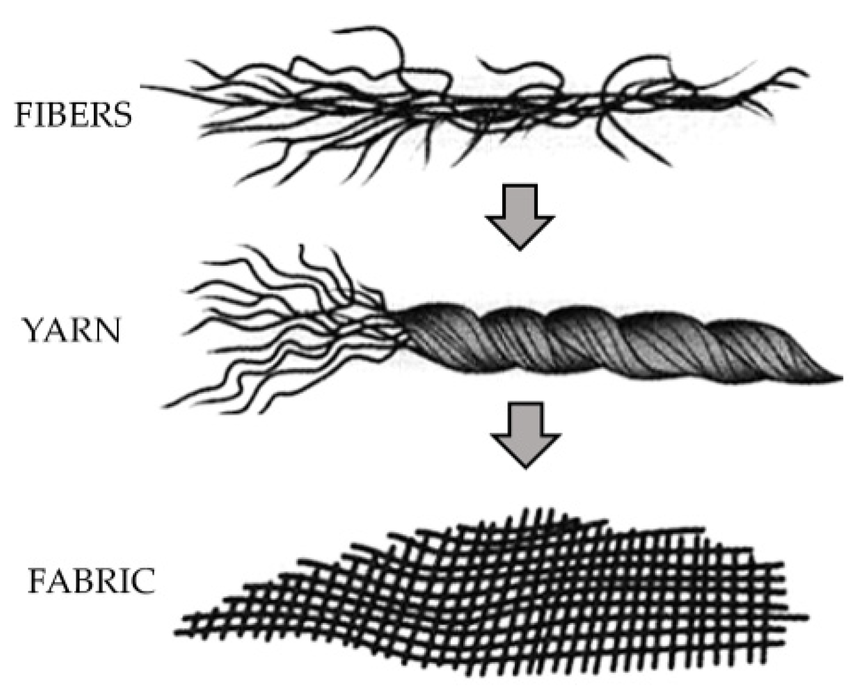
\includegraphics[width=0.6\textwidth]{images/fabric_construction}
            \caption{Construction of Fabric from Fibres}
            \label{fig:fabric_construction}
        \end{figure}
    \item \textbf{Properties derived from fibres and construction:} A fabric's properties (e.g., drape, texture, durability, breathability, warmth) are a result of the types of fibres used, the yarns created from them, and the specific construction method (weave, knit, etc.) \cite{researchgate, hong2024research}.
\end{itemize}

\textbf{Examples of Fabrics:}
\begin{itemize}
    \item Cotton fabric, Silk fabric, Wool fabric, Polyester fabric, Denim, Chiffon, Fleece, Canvas.
\end{itemize}

\newpage

\subsection{Differences Between Fibre and Fabric}
\addcontentsline{toc}{subsection}{Differences Between Fibre and Fabric}

The core distinction lies in their hierarchical position within textile production and their form:

\begin{table}[h!]
    \centering
    \caption{Key Differences Between Fibre and Fabric}
    \label{tab:fibre_fabric_diff}
    \begin{tabular}{l p{5cm} p{5cm}} % Adjust column width for content
        \toprule
        \textbf{Feature} & \textbf{Fibre} & \textbf{Fabric} \\
        \midrule
        \textbf{Definition} & A single, thread-like filament or natural/synthetic substance \cite{researchgate}. & A material produced by weaving, knitting, felting, or bonding fibres/yarns \cite{researchgate, hong2024research}. \\
        \textbf{Form} & Basic, raw, individual component. & Constructed, cohesive, sheet-like material. \\
        \textbf{Stage of Production} & Precursor to yarn. The fundamental unit. & End product of textile formation (from yarn/fibre). \\
        \textbf{Usability} & Not directly used for clothing/products (must be processed) \cite{researchgate}. & Directly usable for making clothing and other textile products. \\
        \textbf{Properties} & Determines inherent characteristics (e.g., raw strength, absorbency) \cite{researchgate}. & Properties result from fibre type \textit{and} construction method (e.g., drape, texture, finished strength) \cite{researchgate, hong2024research}. \\
        \textbf{Analogy} & Think of individual strands of hair. & Think of a piece of cloth woven from those hair strands. \\
        \bottomrule
    \end{tabular}
\end{table}

In essence, fibres are the raw ingredients, while fabrics are the cooked meal, ready for consumption (or in this case, for garment manufacturing). The journey from numerous individual fibres to a usable, textured fabric involves intricate processes that define the look, feel, and performance of the final textile product.